\documentclass[12pt,a4paper]{article}

\usepackage[a4paper,margin=1in]{geometry}
\usepackage{graphicx}
\usepackage{float}
\usepackage{hyperref}
\usepackage{titlesec}
\usepackage{setspace}
\usepackage{color}


\hypersetup{
    colorlinks=true,
    linkcolor=blue,
    urlcolor=blue
}


\title{
\vspace{1cm}


\includegraphics[width=0.25\textwidth]{Image/Logo.png}\\[0.5cm]

{\Large GISMA University of Applied Sciences}\\[0.3cm]
{\Large BSc Computer Science}\\[0.3cm]
{\Large Computer Science Lab}\\[1.5cm]

\rule{\textwidth}{0.5mm}\\[0.6cm]

{\Huge \textbf{Computer Science Portfolio}}\\[0.4cm]

{\Large Individual Project Report}\\[0.6cm]

\rule{\textwidth}{0.5mm}\\[2cm]
}

\author{\Large Aayush Dhami (GH1056547)}

\date{\today}

\begin{document}

\maketitle
\clearpage
\thispagestyle{empty}

\newpage

\tableofcontents

\newpage


\section{Introduction}

This report presents the design, development, and evaluation of my personal Computer Science Portfolio website. The portfolio was created as part of the Computer Science Lab module to showcase my technical skills, academic background, projects, and professional experience.

The website was developed using HTML, CSS, and JavaScript and is hosted using GitHub Pages. The portfolio serves as an online professional profile that can be shared with employers and recruiters.

\vspace{0.5cm}

\textbf{Portfolio Website:}

\url{https://aayushdhami578-sketch.github.io/Portfolio_Web/}

\vspace{0.3cm}

\textbf{GitHub Repository:}

\url{https://github.com/aayushdhami578-sketch/Portfolio_Web}



\section{Portfolio Overview}

The primary objective of this portfolio website is to present my academic 
background, technical skills, projects, and professional experience in a 
structured and professional manner. As a Computer Science student, having 
an online portfolio allows potential employers, recruiters, and academic 
staff to evaluate my abilities beyond a traditional curriculum vitae. The 
portfolio serves as a central location where visitors can learn about my 
education, view my projects, and access my contact information.

The website is organised into five main sections: Home, Portfolio, Resume, 
About Me, and Contact. Each section was designed with a specific purpose 
and contributes to the overall presentation of my professional profile.

The Home section acts as the landing page of the website. It provides a 
simple greeting, introduces me by name, and presents a profile photograph. 
The purpose of this section is to create a positive first impression and 
clearly identify the website as my personal computer science portfolio.

The Portfolio section showcases several academic and personal projects that 
demonstrate my technical abilities. These include the Student Profile 
Management System, Invoice Management System, OTAKUwears Website, and this 
Portfolio Website. Each project is accompanied by a screenshot and a brief 
description to help visitors understand the purpose and technologies 
involved.

The Resume section presents my educational qualifications and professional 
experience. It highlights my studies in Computer Science, foundation year 
education, and teaching experience as a German Language Instructor. This 
section allows visitors to quickly review my academic and professional 
background.

The About Me section provides additional information about my interests, 
career goals, and technical skills. It includes a personal summary and a 
collection of skill badges representing technologies and tools that I have 
experience using, such as HTML, CSS, JavaScript, Python, Git, GitHub, and 
LaTeX.

The Contact section contains my contact details, including GitHub, 
LinkedIn, phone number, and location. It also includes a contact form that 
demonstrates form design and user interface implementation. This section 
enables visitors to find different ways of communicating with me.


The overall structure was intentionally kept simple and easy to navigate. 
Rather than creating multiple webpages, a single-page design was selected 
because it allows users to access all information by scrolling through 
clearly defined sections. This approach provides a smooth user experience 
while maintaining a clean and professional presentation.




\section{Portfolio Website Structure}

The website follows a modern single-page portfolio design.

The design uses a grey colour scheme combined with white text to maintain readability and a professional appearance. Responsive layouts were implemented using CSS Flexbox and Media Queries to ensure compatibility across different screen sizes.

Key design objectives included:

\begin{itemize}
    \item Simple navigation
    \item Professional appearance
    \item Responsive design
    \item Easy access to projects and CV
    \item Clear presentation of information
\end{itemize}

\subsection{Home Page}

The home page introduces visitors to the portfolio and provides a brief professional summary.

\begin{figure}[H]
\centering
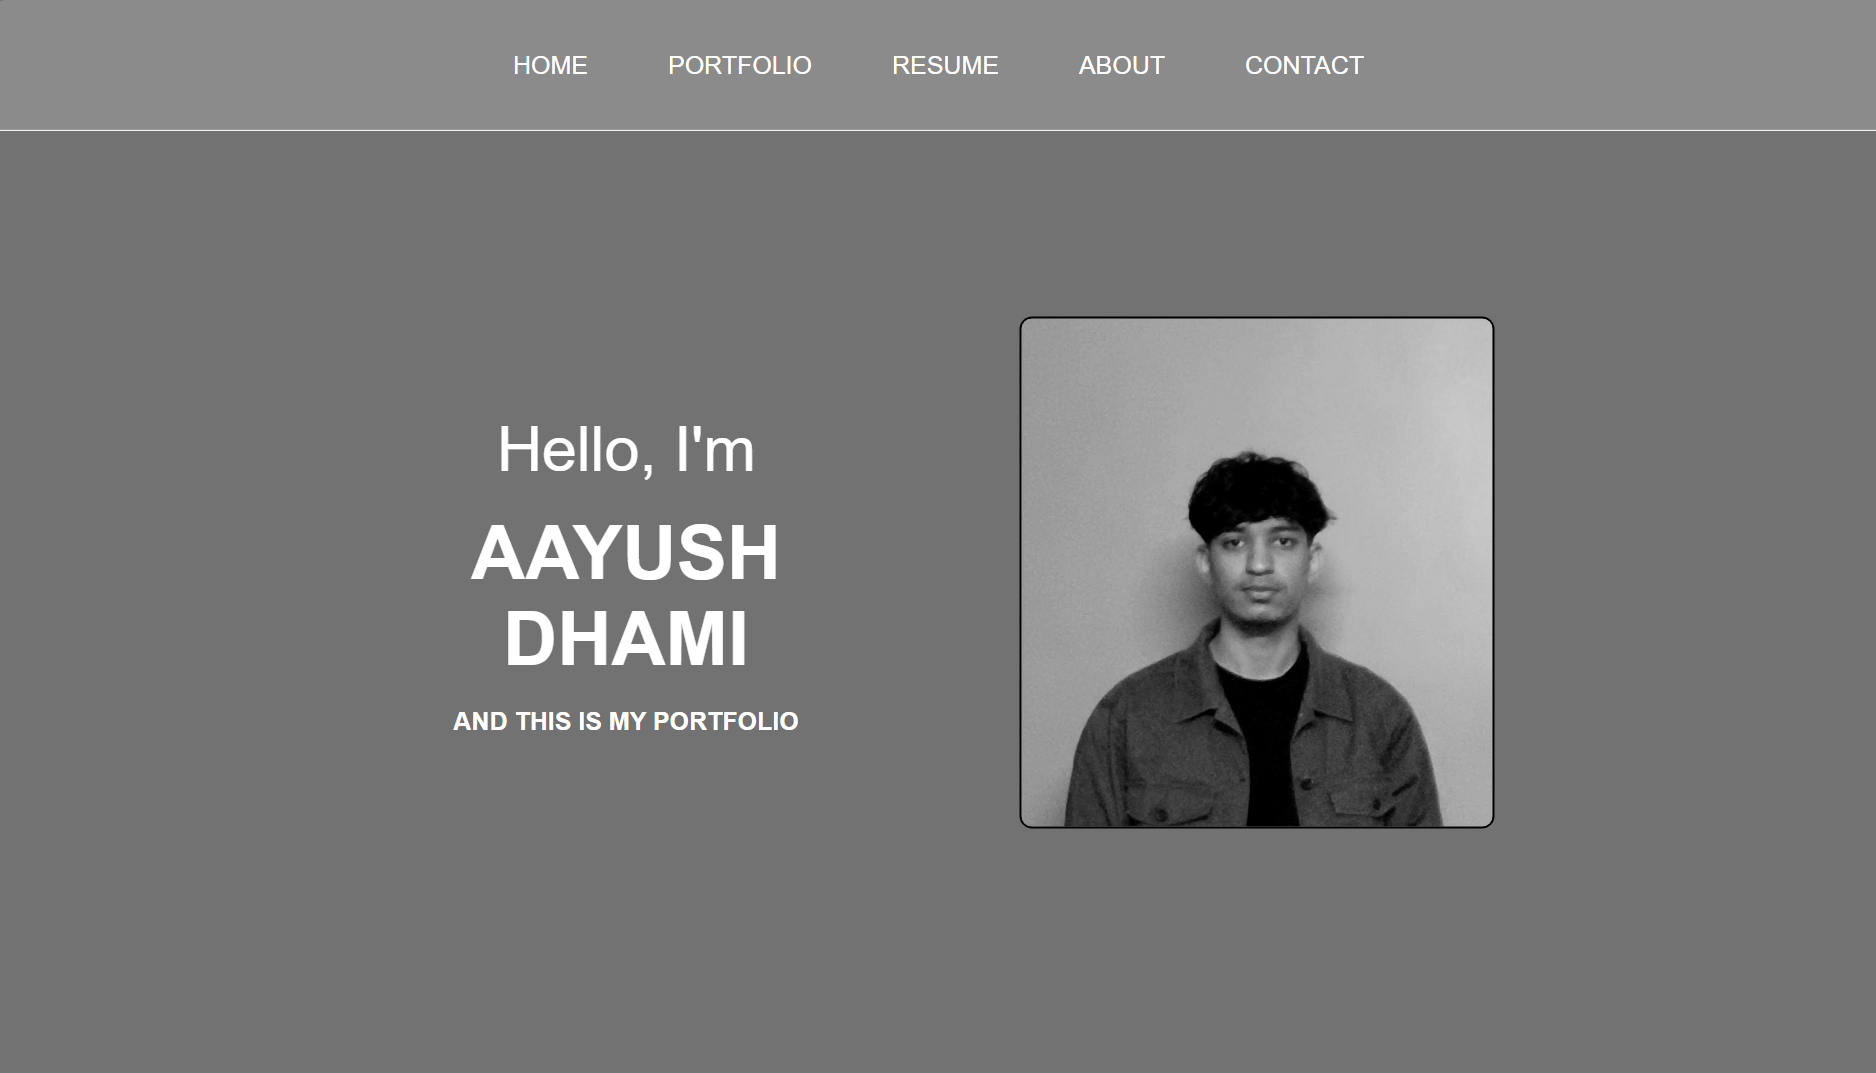
\includegraphics[width=0.9\textwidth]{Image/Home.png}
\caption{Home Page}
\end{figure}



\subsection{Portfolio Section}

This section showcases my technical projects. Each project includes an image, description, technologies used, and links to the source code where appropriate.

Projects included:
\begin{itemize}
  \item Invoice Management System (C++)
  \item Student Profile Management System (Python)
  \item Online Store Website (HTML, CSS, JavaScript)
\end{itemize}


\begin{figure}[H]
\centering
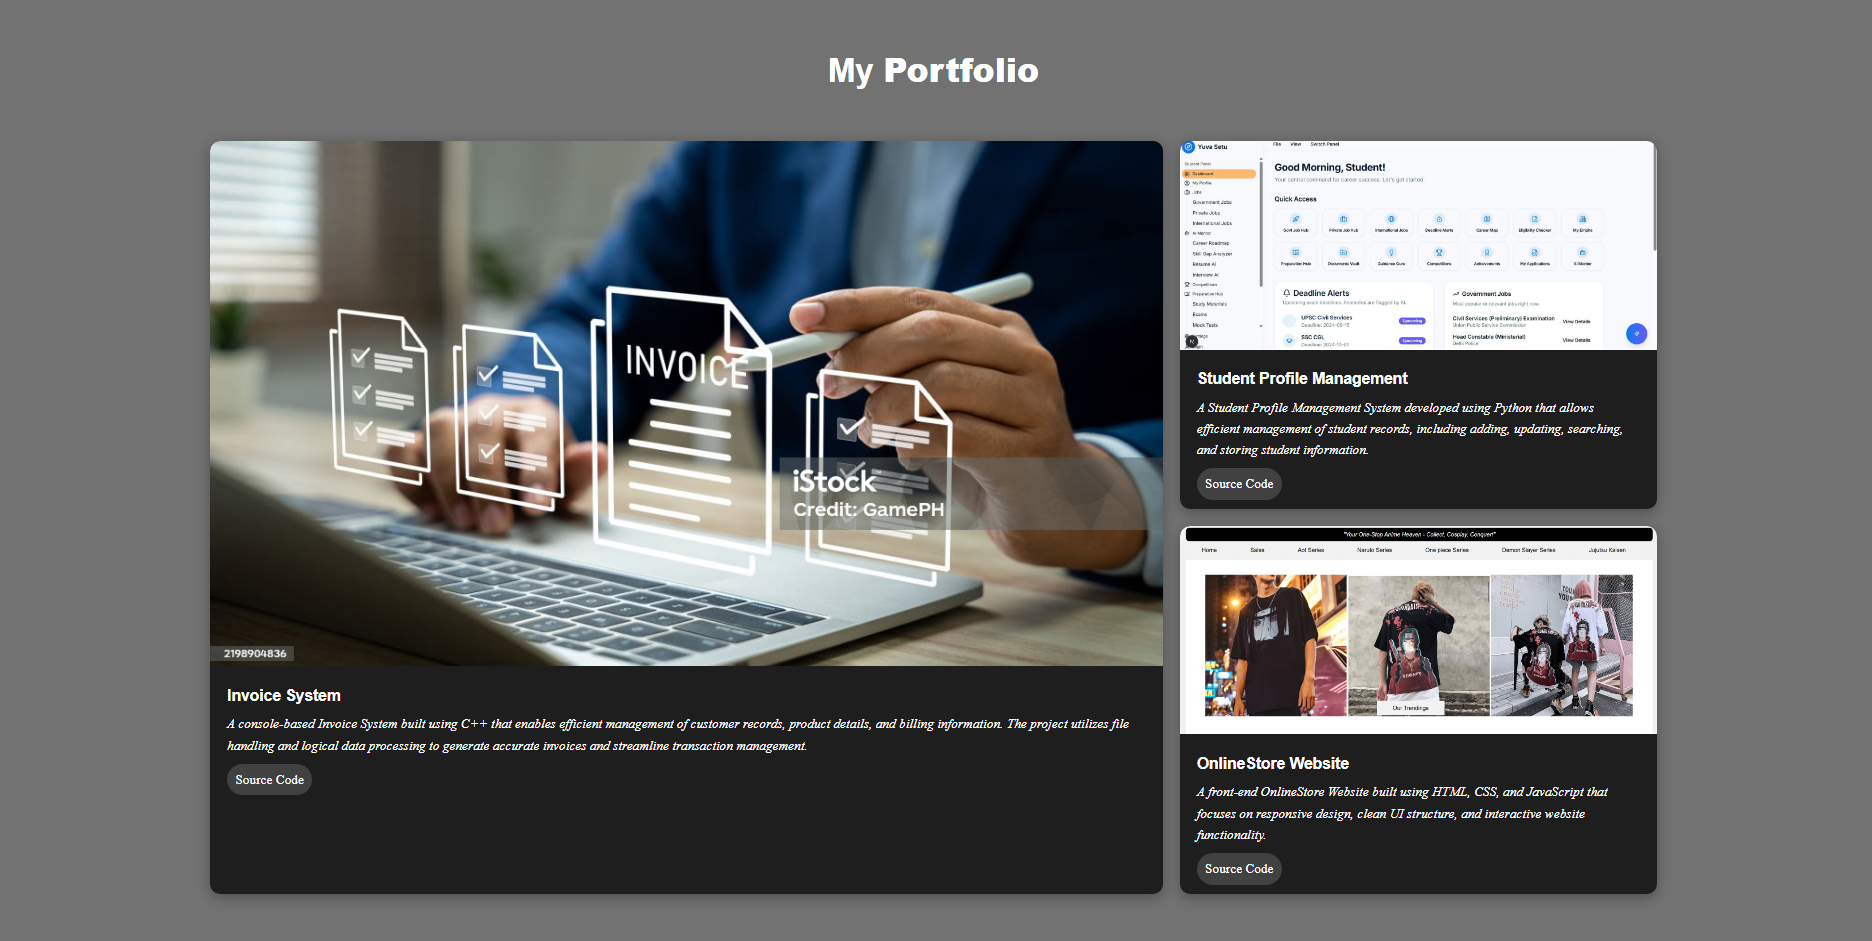
\includegraphics[width=0.9\textwidth]{Image/Portfolio.png}
\caption{Portfolio Projects}
\end{figure}

\subsection{Resume Section}

The Resume section displays my education and work experience.

\begin{figure}[H]
\centering
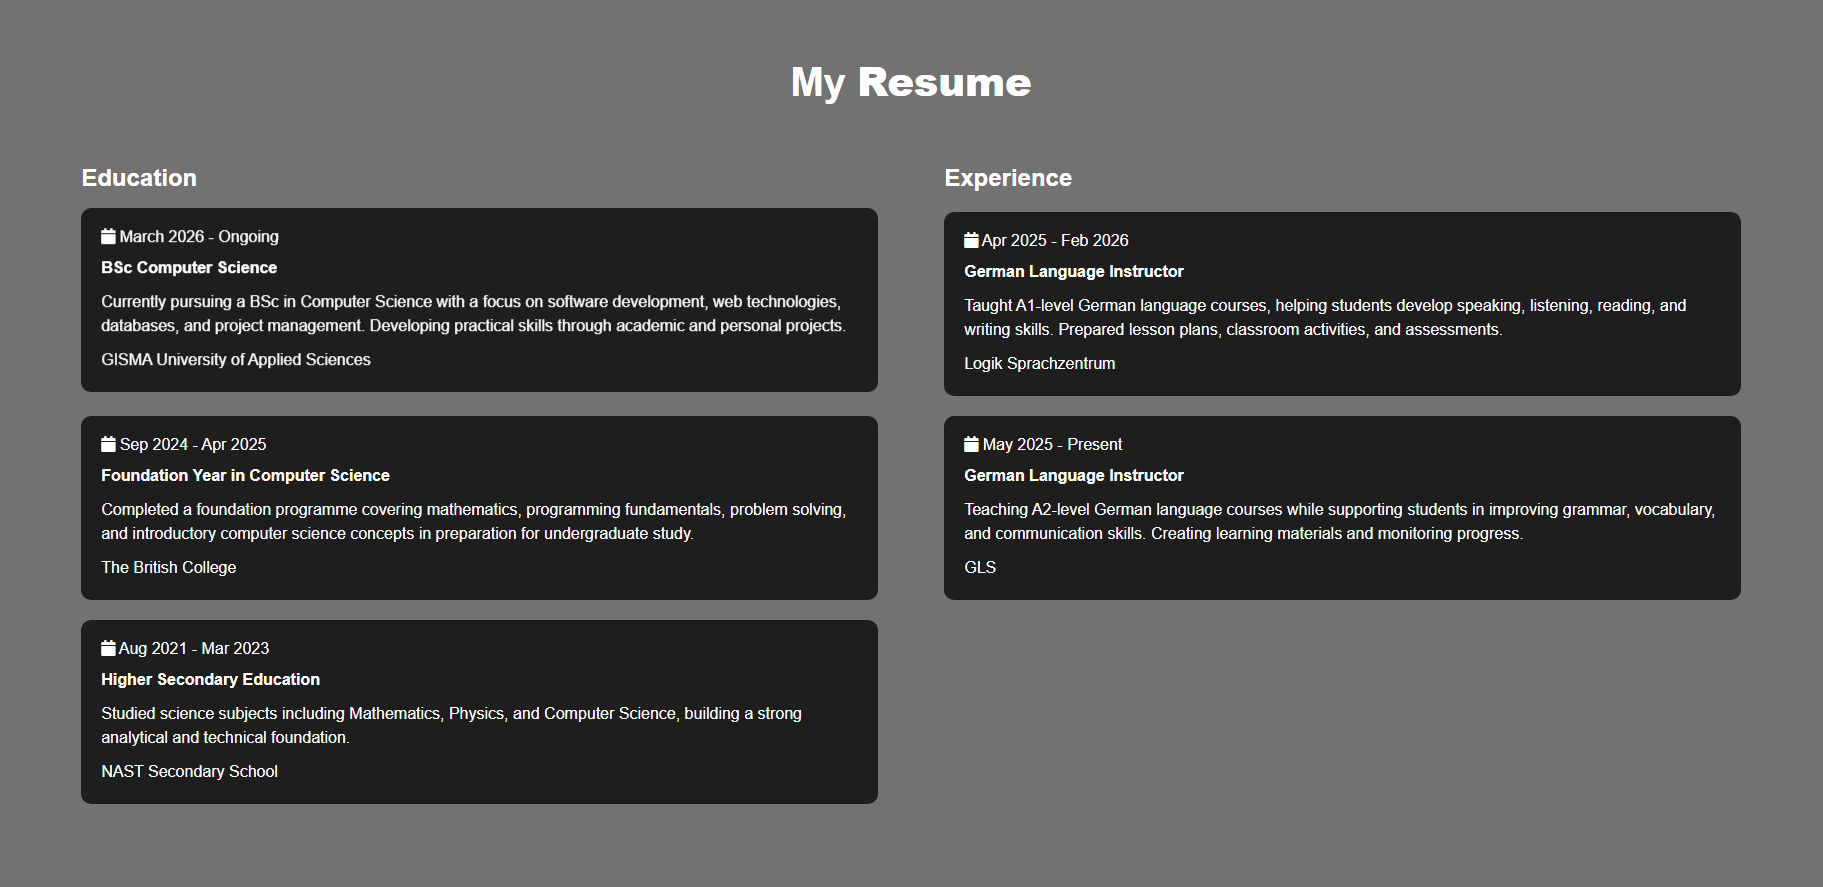
\includegraphics[width=0.9\textwidth]{Image/Resume.png}
\caption{Resume Section}
\end{figure}

\subsection{About Me Section}

This section provides information about my background, interests, and technical skills.

\begin{figure}[H]
\centering
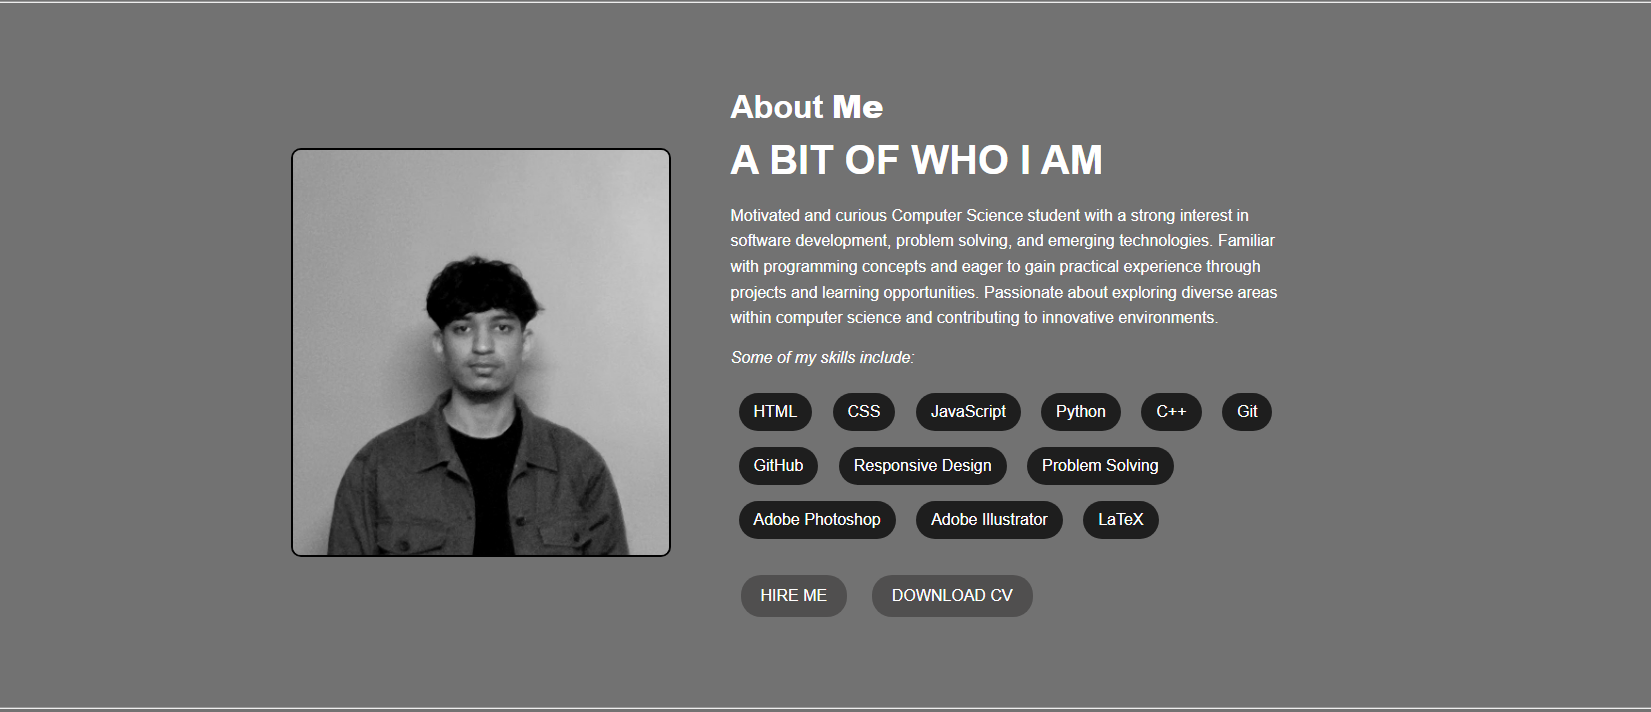
\includegraphics[width=0.9\textwidth]{Image/AboutMe.png}
\caption{About Me Section}
\end{figure}

\subsection{Contact Section}

The contact section allows visitors to access my contact details and submit messages.

\begin{figure}[H]
\centering
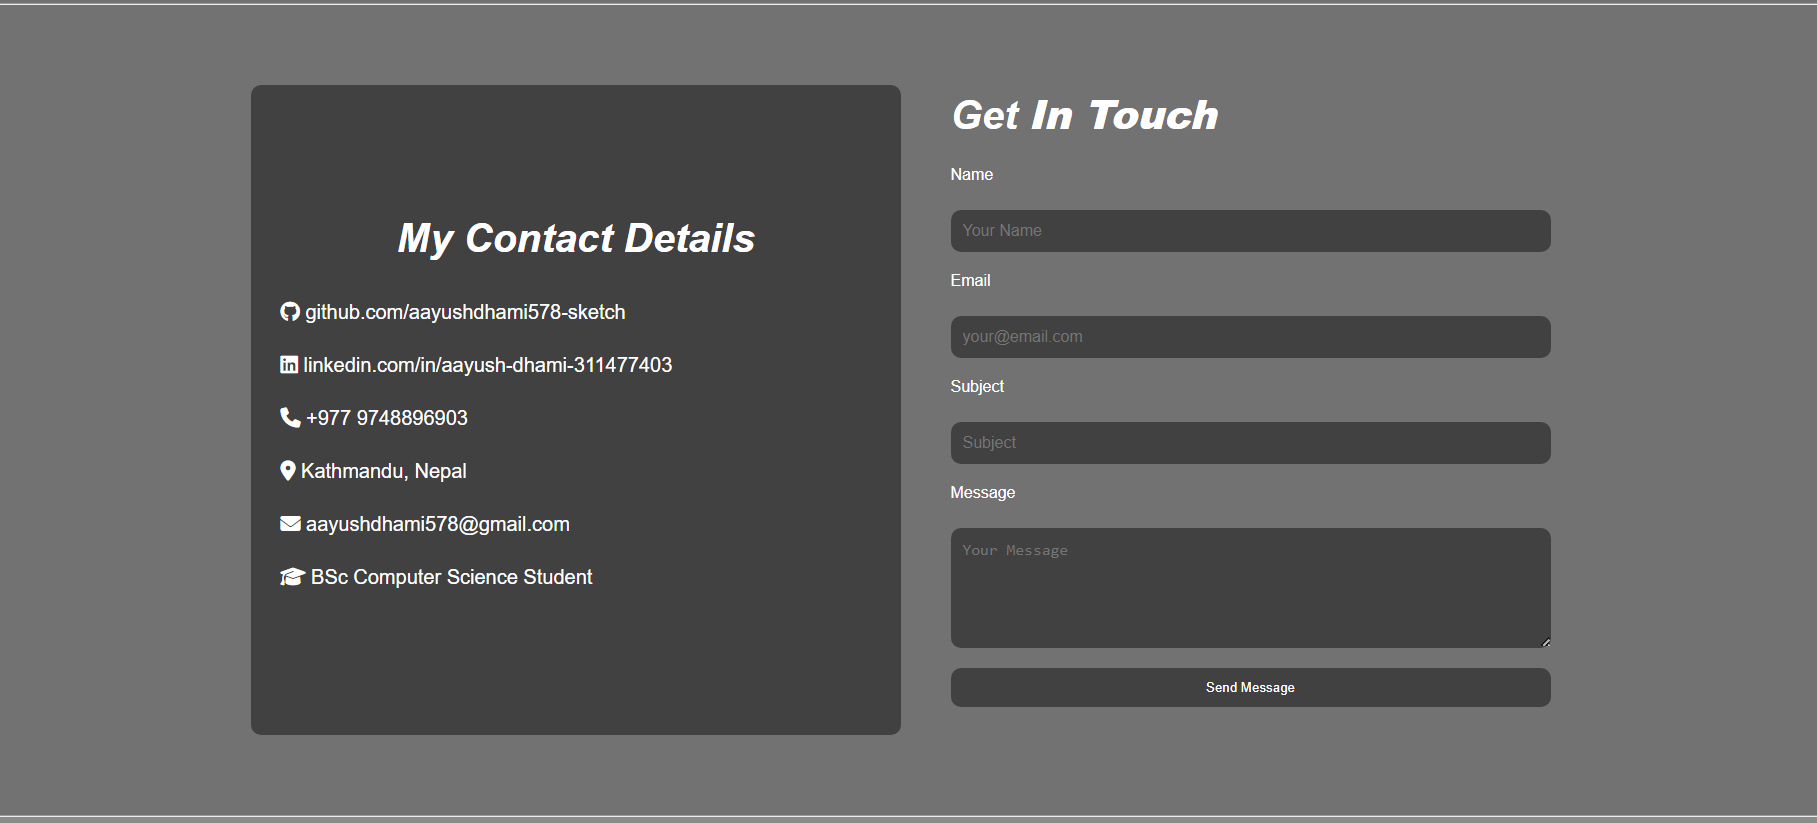
\includegraphics[width=0.9\textwidth]{Image/Contact.png}
\caption{Contact Section}
\end{figure}



\section{Design Decisions}

Several design decisions were made throughout the development of the 
portfolio website to improve usability, readability, responsiveness, and 
overall visual appeal. The objective was to create a professional portfolio 
that presents information clearly while remaining accessible across 
different devices.

\subsection{Colour Scheme}

A dark grey colour palette was selected because it provides a modern and 
professional appearance that is commonly found in technology-related 
websites and portfolios. Dark backgrounds help important content stand out 
while reducing unnecessary visual distractions. White text was used 
throughout the website to maximise readability and provide strong contrast 
against the background. Consistent colours were maintained across all 
sections to create a unified visual identity and improve the overall user 
experience.

\subsection{Navigation Bar}

A sticky navigation bar was implemented to improve website navigation. The 
navigation menu remains visible while users scroll through the page, 
allowing quick access to different sections without needing to return to 
the top of the website. JavaScript was used to highlight the currently 
active section, providing visual feedback and helping users understand 
their location within the portfolio. This improves usability, particularly 
on longer single-page websites.

\subsection{Responsive Layout}

One of the most important design considerations was ensuring that the 
website functioned correctly on different screen sizes. During the initial 
stages of development, some sections relied on fixed positioning and 
dimensions. While the layout appeared correct on my personal computer, 
testing revealed that the website became distorted on devices with 
different screen resolutions.

To address this issue, the layout was redesigned using CSS Flexbox, CSS 
Grid, and Media Queries. Flexbox was used to organise content into flexible 
rows and columns, while Grid was used to structure the project showcase 
section. Media Queries were implemented to adjust layouts automatically on 
smaller screens. These changes significantly improved responsiveness and 
ensured that the portfolio remained usable on desktop computers, tablets, 
and mobile devices.

\subsection{Project Showcase Layout}

The Portfolio section uses a grid-based layout to display projects in a 
visually organised manner. A larger project card was used to highlight a 
featured project, while smaller cards were used for supporting projects. 
This creates a clear visual hierarchy and helps direct the visitor's 
attention toward key pieces of work. Each project includes a screenshot and 
description, allowing visitors to quickly understand the purpose and 
functionality of the showcased work.



\section{GitHub Repository Structure}

The project is managed using Git and hosted on GitHub. Version control was 
used throughout development to track changes and maintain project history.

The repository contains:

\begin{itemize}
\item index.html – Main website structure
\item style.css – Website styling and layout
\item script.js – Interactive website functionality
\item Image folder – Project screenshots and profile images
\item CV.pdf – Curriculum Vitae created using LaTeX
\item  README.md – Repository documentation
\end{itemize}
This structure ensures that content, styling, and functionality remain 
separated and easy to manage.

\begin{figure}[H]
\centering
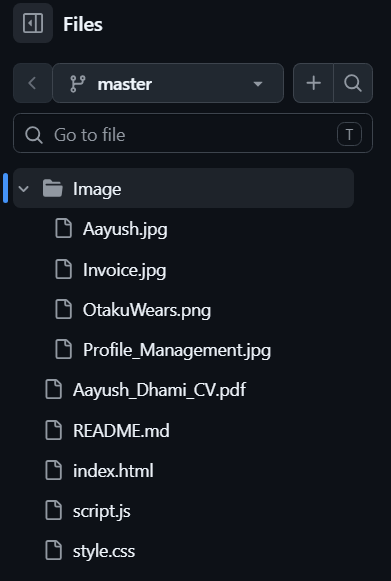
\includegraphics[width=0.6\textwidth,height=15cm]{Image/Github.png}
\caption{GitHub Repository Structure}
\end{figure}



\section{Technologies Used}

Several technologies were used during development:

\begin{itemize}
    \item HTML:
    HTML was used to create the structure of the website, including 
    sections, navigation, project cards, and content.
    \item CSS: 
    CSS was used to style the website and create layouts using Flexbox and 
    Grid. It was also used to implement animations, hover effects, and 
    responsive design.
    \item JavaScript:
    JavaScript was used to improve user interaction, including the active 
    navigation highlighting feature and other dynamic elements.
    \item Git and GitHub:
    Git was used for version control, while GitHub was used to host the 
    repository and publish the portfolio through GitHub Pages.
    \item LaTeX :
    LaTeX was used to create a professional Curriculum Vitae. The CV was 
    included within the repository and linked from the portfolio website.
    \item Visual Studio Code :
    Visual Studio Code was used as the development environment.
\end{itemize}


These projects demonstrate skills in programming, web development, version 
control, and software design.


\section{Challenges Encountered During Development}

Several challenges were encountered throughout the development process. One 
of the first challenges involved deploying the website using GitHub Pages. 
Although the website functioned correctly in the local development 
environment, certain images failed to appear after deployment. After 
investigating the issue, it was discovered that file path names were not 
matching the exact capitalisation of the folder names stored in the 
repository. Because GitHub Pages operates on a Linux-based system, file 
paths are case-sensitive. Correcting the folder names resolved the problem.


Another challenge involved creating a responsive layout. Initially, many 
elements relied on fixed dimensions and absolute positioning. This approach 
produced acceptable results on a single device but created problems when 
viewed on different screen sizes. Through testing and experimentation, the 
layout was restructured using Flexbox and Media Queries. This significantly 
improved responsiveness and reduced layout inconsistencies.


Version control also presented a learning opportunity. Throughout 
development, Git and GitHub were used to manage source code and track 
changes. Working with commits, branches, and repository updates improved my 
understanding of software development workflows and highlighted the 
importance of maintaining organised project histories.


\section{Evaluation and Reflection}

\subsection{Strengths}

One of the strongest aspects of the portfolio is its organisation. 
Information is grouped logically into clearly defined sections, allowing 
visitors to navigate efficiently. The use of GitHub Pages provides a 
reliable and publicly accessible hosting platform, while responsive design 
techniques ensure compatibility across different devices.

The project also demonstrates practical knowledge of HTML, CSS, JavaScript, 
Git, GitHub, and LaTeX. The integration of these technologies highlights 
both technical and organisational skills that are valuable within software 
development environments.

\subsection{Weaknesses}

Despite these strengths, several limitations remain. The contact form 
currently lacks backend functionality and therefore cannot process user 
submissions. Additionally, JavaScript functionality is relatively limited 
and could be expanded to create a more interactive user experience. The 
portfolio would also benefit from the inclusion of additional projects that 
demonstrate more advanced programming concepts.

\subsection{Future Improvements}

Although the portfolio successfully achieves its primary objectives, 
several improvements could be implemented in future versions. One potential 
enhancement would be the addition of more software development projects. 
Including larger and more technically advanced projects would provide visitors
with a broader understanding of my programming abilities and problem-solving skills.
Another important improvement would be the implementation of a fully functional
backend for the contact form. At present, the form serves primarily as a visual
component and does not process user submissions. Integrating a backend service would 
allow visitors to send messages directly through the website.
Additional interactive features could also improve the user experience. 
Examples include project filtering, animations, theme customisation, 
and a dark/light mode switch. These features would increase engagement while 
demonstrating additional front-end development skills.
Finally, the website could be expanded with a dedicated blog section where 
technical learning experiences, project updates, and programming insights could be shared.
This would allow the portfolio to evolve beyond a static website and become a platform 
for continuous professional development.


\section{Conclusion}

This project successfully demonstrates my ability to design, develop, and 
deploy a professional computer science portfolio website. The portfolio 
showcases my educational background, technical skills, and projects while 
providing an online presence that can be shared with employers and 
recruiters.

The project also allowed me to gain practical experience with web 
development, Git version control, GitHub Pages deployment, and technical 
documentation using LaTeX.



\section{References}

\begin{itemize}

\item Overleaf (2026) \textit{Clean CV Template}. Available at:
\url{https://www.overleaf.com/latex/templates/clean-cv-template/rcqjkxnfsmnz}
(Accessed: 25 June 2026).

\item ThemeWagon (2026) \textit{Rezume Portfolio Template}. Available at:
\url{https://themewagon.github.io/rezume/}
(Accessed: 25 June 2026).

\end{itemize}

\end{document}